\documentclass[10pt, conference, compsocconf]{IEEEtran}

\usepackage{cite}
\usepackage[pdftex]{graphicx}
\usepackage[cmex10]{amsmath}
\usepackage{algorithmic}
\usepackage{array}

\usepackage{mdwmath}
\usepackage{mdwtab}


\usepackage{eqparbox}
\usepackage[caption=false,font=footnotesize]{subfig}
\usepackage{fixltx2e}
%\usepackage{stfloats}
\usepackage{url}
\usepackage{amssymb}
\usepackage{filecontents}
\usepackage{comment}
\usepackage{url}
\usepackage{balance}
\usepackage{booktabs}
\usepackage[linesnumbered,ruled,vlined]{algorithm2e}

\usepackage{lipsum}
\setlength{\intextsep}{0pt}
\setlength{\textfloatsep}{0pt}% Remove \textfloatsep

% correct bad hyphenation here
\hyphenation{op-tical net-works semi-conduc-tor}

\newtheorem{theorem}{Theorem}
\newtheorem{lemma}{Lemma}

\begin{document}
%
% paper title
% can use linebreaks \\ within to get better formatting as desired
\title{On Speeding-up Parallel Jacobi Iterations for SVDs}


% author names and affiliations
% use a multiple column layout for up to two different
% affiliations

\author{\IEEEauthorblockN{Soumitra Pal \qquad Sudipta Pathak \qquad Sanguthevar Rajasekaran}
\IEEEauthorblockA{Computer Science and Engineering, University of Connecticut\\
371 Fairfield Road, Storrs, CT 06269, USA\\
\texttt{\small \em \{mitra@,sudipta.pathak@,rajasek@engr.\}uconn.edu}}}

% conference papers do not typically use \thanks and this command
% is locked out in conference mode. If really needed, such as for
% the acknowledgment of grants, issue a \IEEEoverridecommandlockouts
% after \documentclass

% for over three affiliations, or if they all won't fit within the width
% of the page, use this alternative format:
% 
%\author{\IEEEauthorblockN{Michael Shell\IEEEauthorrefmark{1},
%Homer Simpson\IEEEauthorrefmark{2},
%James Kirk\IEEEauthorrefmark{3}, 
%Montgomery Scott\IEEEauthorrefmark{3} and
%Eldon Tyrell\IEEEauthorrefmark{4}}
%\IEEEauthorblockA{\IEEEauthorrefmark{1}School of Electrical and Computer Engineering\\
%Georgia Institute of Technology,
%Atlanta, Georgia 30332--0250\\ Email: see http://www.michaelshell.org/contact.html}
%\IEEEauthorblockA{\IEEEauthorrefmark{2}Twentieth Century Fox, Springfield, USA\\
%Email: homer@thesimpsons.com}
%\IEEEauthorblockA{\IEEEauthorrefmark{3}Starfleet Academy, San Francisco, California 96678-2391\\
%Telephone: (800) 555--1212, Fax: (888) 555--1212}
%\IEEEauthorblockA{\IEEEauthorrefmark{4}Tyrell Inc., 123 Replicant Street, Los Angeles, California 90210--4321}}



% make the title area
\maketitle


\begin{abstract}
We live in an era of big data and the analysis of these data is becoming a bottleneck in many domains including biology and the internet. To make these analyses feasible in practice, we need efficient data reduction algorithms. The Singular Value Decomposition (SVD) is a data reduction technique that has been used in many different applications. For example, SVDs have been extensively used in text analysis. The best known sequential algorithms for the computation of SVDs take cubic time which may not be acceptable in practice. As a result, many parallel algorithms have been proposed in the literature. There are two kinds of algorithms for SVD, namely, QR decomposition and Jacobi iterations. Researchers have found out that even though QR is sequentially faster than Jacobi iterations, QR is difficult to parallelize. As a result, most of the parallel algorithms in the literature are based on Jacobi iterations. JRS is a relaxation of the classical Jacobi algorithm and has been shown to be very effective in parallel. In this paper we propose a novel variant of the classical Jacobi algorithm that is more efficient than the JRS algorithm. Our experimental results confirm this assertion. The key idea behind our algorithm is to select the pivot elements for each sweep appropriately. 
%We also provide a convergence proof for our new algorithm. 
We also show how to efficiently implement our algorithm on such parallel models as the PRAM and the mesh. 
\end{abstract}

\begin{IEEEkeywords}
SVD; Jacobi iterations; JRS; parallel algorithms
\end{IEEEkeywords}


% For peer review papers, you can put extra information on the cover
% page as needed:
% \ifCLASSOPTIONpeerreview
% \begin{center} \bfseries EDICS Category: 3-BBND \end{center}
% \fi
%
% For peerreview papers, this IEEEtran command inserts a page break and
% creates the second title. It will be ignored for other modes.
\IEEEpeerreviewmaketitle



\section{Introduction}
\label{sec:intro}

Singular Value Decomposition (SVD) is a fundamental computational problem in linear algebra and it has applications in various computational science and engineering areas. For example, it is widely used in areas such as statistics where it is directly related to principal component analysis, in signal processing and pattern recognition as an essential filtering tool, and in control systems. Recently, it is used as one of the fundamental steps in many machine learning applications such as least square regressions, information retrieval and so on. With the advent of BigData, it has become essential to process data matrices with thousands of rows and columns in real time. The SVD is one of the data reduction techniques. Hence, there is a strong need for efficient sequential and parallel algorithms for the SVD.

SVD takes as input a matrix $A \in \mathbb{F}^{m \times n}$ where $\mathbb{F}$ could be the field of real ($\mathbb{R}$) or complex ($\mathbb{C}$) numbers and outputs three matrices $U, S, V$ such that $A = USV^T$, where $U \in \mathbb{F}^{m \times m}$, $V \in \mathbb{F}^{n \times n}$ are orthogonal matrices (i.e. $U^TU = I_m$, $V^TV = I_n$) and $S \in \mathbb{R}^{m \times n}$ is a diagonal matrix. If $S = diag(\sigma_1, \sigma_2,......\sigma_{\min\{m,n\}})$, then the diagonal elements $\sigma_i$s are called the singular values of $A$. The columns of $U$ and $V$ are referred to as the left and right singular vectors, respectively. Without loss of generality, we assume that $m \ge n$. We also assume that the input matrices are real, the algorithms in this paper can be easily extended to complex matrices. 

There are various methods of computing the SVD~\cite{golub2012matrix}. The most commonly used algorithms for dense matrices, which we consider in this paper, can be classified as \emph{QR-based} and \emph{Jacobi-based}. The QR-based algorithms work in two stages. In the first stage the input matrix is converted to a band matrix (bidiagonal, tridiagonal, and so on) using factorizations such as Cholesky, LU and QR. In the final stage the band matrix is converted to a diagonal form to obtain the singular values. The singular vectors are also computed accordingly. In the sequential setting, the QR based methods are more frequently used as they are faster than the sequential Jacobi based methods. However, Jacobi-based methods are known to be more accurate~\cite{demmel1992jacobi} and also have a higher degree of potential parallelism. Though there are parallel implementations of QR based algorithms in an out-of-core setting~\cite{grimes1987solution, grimes1988solution} as well as in homogeneous multi-core setting~\cite{haidar2013improved}, our focus in this paper  is on designing faster parallel implementations of the Jacobi based algorithms.

There are two different variations of the Jacobi based algorithms, \emph{one-sided} and \emph{two-sided}. The two sided Jacobi algorithms are applicable only when $A$ is symmetric and $m=n$. The basic idea of a two sided Jacobi algorithm is as follows. Using a series of plane rotation matrices $U_1, U_2, \ldots, U_t$, the symmetric matrix $A$ is converted a diagonal matrix $S = U_t \ldots U_2 U_1 A U^T_1 U^T_2 \ldots U^T_t$. The left and right singular vectors are given by $U=V=U_1U_2,\ldots,U_t$. The basic idea of the one-sided Jacobi algorithms proposed by Hestenes~\cite{hestenes1958inversion} is as follows. Using a series of plane rotation matrices $V_1, V_2, \ldots, V_t$ the input matrix $A$ is first converted to a matrix $B=AV_1V_2\ldots V_t$ such that the columns of $B$ are orthogonal. The decomposition $B = US$ gives us the required left singular vectors and the singular values respectively, where $U$ is obtained by normalizing the columns of $B$ (keeping null columns unchanged) and the norm of $i$th column of $B$ gives $S_{ii}$ of the diagonal matrix $S$. The right singular vectors are the columns of $V=V_1V_2,\ldots,V_t$. As the rotation matrices $V_i$s are orthogonal, $V$ is also orthogonal and hence $AV = B = US$ implies $A = USV^T$.

Each of the plane rotation matrices $V_i$ corresponds to a pair of columns $(j,k)$ where the rotation is on the plane going through the $j$th and the $k$th axes. We assume $j<k$ and call such a pair $(j,k)$ a \emph{pivot}.  In the traditional Jacobi algorithms the rotations are divided among \emph{sweeps}, in each sweep all possible ${n \choose 2}$ pivots are used. For the two-sided Jacobi, the rotation using the pivot $(j,k)$ annihilates the off diagonal entries $a_{jk}, a_{kj}$ to $0$. However, either of $a_{jk}, a_{kj}$ may again become non-orthogonal due to some later pivot involving $j,k$ in the same sweep. Hence multiple sweeps are required. As a test for convergence, we could check if the Frobenius norm of the off-diagonal entries of $A$ fall below a certain tolerance. For the one-sided Jacobi, pivoting $(j,k)$ ensures that the columns $a_j,a_k$ become mutually orthogonal after the rotation. Here too, multiple sweeps may be required as the columns may again become non-orthogonal due to some later pivot. For convergence, we could count how many times in any sweep the dot-product $a_j^{T}a_k$ fell below a certain tolerance and the algorithm is terminated when the count reached $n(n-1)/2$. It is believed that the number $S$ of sweeps needed for the convergence of the sequential one-sided and two-sided Jacobi algorithms is $O(\log n)$~\cite{golub2012matrix}.  

It turns out that the order in which the pivots are applied in a sweep has a significant effect on the number of sweeps required for convergence. Mainly two different orders are used. In the classic Jacobi algorithm~\cite{golub2012matrix}, each rotation chooses the pivot $(j,k)$ with the maximum absolute value of $a_{jk}$ in the two-sided Jacobi and the maximum value of the dot-product $a_j^{T}a_k$ in the one-sided Jacobi. However, searching for this element is computationally expensive. Cyclic Jacobi algorithms trade off this computation with slower convergence and use the pivots in the order $(1,2), (1,3), \ldots, (1,n),$ $(2,3), (2,4), \ldots, (2,n), \ldots, (n{-}1,n)$.  It can be shown that after each sweep in two-sided Jacobi the Frobenius norm of the off-diagonal entries reduces monotonically and hence the algorithm converges. For the one-sided Jacobi the sum of dot-products of all pairs of columns reduces in each sweep.

Many pivots in a sweep are independent of each other and hence the corresponding rotations can be applied in parallel. In fact the sweeps can be divided into $(n-1)$ \emph{subsweeps} each containing $n/2$ independent pivots and all rotations in a subsweep can be applied in parallel. There are many ways of dividing the pivots in a subsweep. A simple round-robin based ordering is given in~\cite{golub2012matrix}. However, it turns out that more clever pivot ordering improves performance by reducing the total number of sweeps required for convergence~\cite{bevcka2002dynamic}.

\subsection{Contributions}

In this paper we introduce a novel algorithm for parallel computation of SVDs. Our algorithm is faster than the classical Jacobi algorithm in sequence. This algorithm uses the idea of picking the pivots in the order of maximum absolute value of $a_{jk}$ in two-sided Jacobi and of $a_j^T a_k$ in one-sided Jacobi. However, to reduce the high computational cost of searching for the maximum before each rotation, the algorithm uses two relaxations: 1) instead of searching for the maximum before each iteration, the pivots are sorted in descending values of $a_{jk}$ or $a_j^T a_k$ at the beginning of a sweep and the pivots are applied in this order, and 2) in each sweep only the top $\frac{1}{\tau}$ fraction of the pivots are selected and they are applied in the sorted order. We call this JTS (Jacobi Target Selection) scheme hereafter. Our contributions are as follows. Firstly we show using a `simulation' based technique~\cite{rajasekaran2008relaxation} that the JTS scheme significantly reduces the number of sweeps required to reach convergence. Secondly we give a `real' implementation of our ideas in a one-sided Jacobi algorithm based on the source code from Gnu Scientific Library~\cite{galassi1996gnu}. We also give a parallel version of this real implementation in the shared memory multi-core setting. Finally we discuss the implementation of JTS scheme on various models of parallel computing such as the mesh and the PRAM.
 

The remainder of the paper is organized as follows: In Section~\ref{sec:prevwork}, we survey the previous work on Jacobi-SVD algorithm.  Section~\ref{sec:jts} describes our new JTS algorithm. In Section~\ref{sec:results}, we show experimental results. Section~\ref{sec:other} discusses implementations of our new algorithms in different models of parallel computing. Finally, we provide some concluding remarks in Section~\ref{sec:conclude}.

%\vspace*{-0.1in}

\section{A Survey of Basic Ideas}
\label{sec:prevwork}

Most existing parallel algorithms for SVD are based on the Jacobi iterations. At the heart of these iterations is the Jacobi rotation (also known as Givens rotation~\cite{golub2012matrix}). A rotation of angle $\theta$ in the plane going through the axes $j,k$ can be represented as the following matrix:
%\begin{figure}
\begin{align}
  J(j,k,\theta) &= \left( \begin{array}{ccccccc} 
  1 & \cdots & 0 & \cdots & 0 & \cdots & 0 \\
  \vdots & \ddots & \vdots & & \vdots & & \vdots \\
  0 & \cdots & c & \cdots & s & \cdots & 0 \\
  \vdots & & \vdots & \ddots  & \vdots & & \vdots \\
  0 & \cdots & -s & \cdots & c & \cdots & 0 \\
  \vdots & & \vdots & & \vdots  & \ddots  & \vdots \\
  0 & \cdots & 0 & \cdots & 0 & \cdots & 1
\end{array} \right)
\begin{array}{l}
  \\
  j \\
  \\
  k
  \\
  \\
\end{array} \\
& \begin{array}{ccccccc}
 \qquad &\qquad & j & \qquad & k & &
\end{array} \label{eq:rotation}
\end{align}
%\end{figure}
where $c=\cos \theta$ and $s=\sin \theta$. It is easy to verify that $J^T J = I$, so the Jacobi rotation is an orthogonal transformation.

\subsection{Sequential Jacobi algorithms}
\label{sec:seqalgo}

The two-sided Jacobi algorithms attempt to diagonalize the input matrix $A$ by applying a series of Jacobi rotations of the form $B {=} J^T A J$. It can be easily verified that if $A$ is symmetric then $B$ is also symmetric. The effect of the rotation on $b_{jj}, b_{jk}, b_{kj}, b_{kk}$ can be written as follows:
\begin{align}
\setlength{\arraycolsep}{2.5pt}
  \left(\begin{array}{cc}
    b_{jj} & b_{jk} \\
    b_{kj} & b_{kk}
  \end{array} \right)
  =
  \left(\begin{array}{cc}
    c & s \\
    -s & c
  \end{array} \right)^T
  \left(\begin{array}{cc}
    a_{jj} & a_{jk} \\
    a_{kj} & a_{kk}
  \end{array} \right)
  \left(\begin{array}{cc}
    c & s \\
    -s & c
  \end{array} \right). \nonumber
\end{align}
Suppose we need to annihilate the element $b_{jk}$ (by symmetry $b_{kj}$ too). Solving for $b_{jk} {=} b_{kj} {=} 0$ and taking the smaller root~\cite{golub2012matrix}, gives 
\begin{align}
  c &= \frac{1}{\sqrt{1+t^2}}, & s&=tc, \qquad \text{where} \nonumber \\
  t &= \frac{sign(\gamma)}{|\gamma|+\sqrt{\gamma^2+1}}, & \text{and} \quad \gamma &{=} \frac{a_{kk} {-} a_{jj}}{2a_{jk}}. \nonumber
\end{align}

The one-sided Jacobi algorithm, also called Hestenes–Jacobi algorithm~\cite{hestenes1958inversion}, converts the input matrix $A$ to a orthogonal matrix $B$ using a series of Jacobi rotations of the form $B = A J$. The rotation affects only the columns $j,k$ and can be written in the following matrix notation:
\begin{align}
\setlength{\arraycolsep}{2.5pt}
  \left(\begin{array}{cc}
    b_{j} & b_{k} 
  \end{array} \right)
  =
  \left(\begin{array}{cc}
    a_{j} & a_{k} 
  \end{array} \right)
  \left(\begin{array}{cc}
    c & s \\
    -s & c
  \end{array} \right). \nonumber
\end{align}
The two columns would be orthogonalized if $b_j^T b_k = 0$. Thus solving for $b_{j}^T b_{k} = 0$ gives us 
\begin{align}
  c &= \frac{1}{\sqrt{1+t^2}}, & s&=tc, \qquad \text{where} \nonumber \\
  t &= \frac{sign(\gamma)}{|\gamma|+\sqrt{\gamma^2+1}}, & \text{and} \quad \gamma &= \frac{a_k^T a_k - a_j^T a_j}{2a_j^Ta_k}.
  \label{eq:onesided}
\end{align}
There is a close similarity between the one-sided and the two-sided versions as the one-sided algorithm could be thought of as applying the two-sided algorithm on the symmetric matrix $C = A^TA$. In the rest of the paper we will refer to the one-sided algorithm only as it handles more general matrices and is mostly used in the literature.

The convergence of the one-sided Jacobi algorithm can be shown by the fact that after each iteration the Frobenius norm of the off-diagonal elements of $C$ reduces by a positive quantity and eventually $C$ becomes diagonal. This implies that the columns of $A$ have become orthogonal. The original algorithm by Hestenes~\cite{hestenes1958inversion} also maintains the condition that 
\begin{align}
  ||a_j|| \ge ||a_k|| \qquad \text{for} \; j<k. \label{eq:cond1}
\end{align}
When the cyclic pivot ordering is used, this ensures that in the final output the singular values will be sorted in a non-increasing order. Nash~\cite{nash1975one} gave a faster implementation with two modifications: (i) a rotation is applied only if in addition to~\eqref{eq:cond1} the following condition too holds
\begin{align}
  ||b_j||^2 - ||a_j||^2 = ||a_k||^2 - ||b_k||^2 \ge 0 \label{eq:cond2}
\end{align}
and (ii) the algorithm is stopped if for all possible pivots $(j,k)$ in a sweep, the quantity $\frac{a_j^Ta_k}{(a_j^Ta_j)(a_k^Ta_k)}$ falls below a tolerance level.

\subsection{Parallel Jacobi algorithms}
\label{sec:paralgo}
% \vspace*{-0.1in}
 
The Jacobi algorithm has an inherent parallelism in the sense that many of the ${n \choose 2}$ pivots are independent of each other and hence the rotations for them can be applied in parallel. More precisely the pivots can be divided into $(n{-}1)$ subsweeps and in each subsweep $n/2$ independent pivots can be targeted for rotation in parallel. This applies to both two-sided and one-sided Jacobi algorithms. In the original Hestenes algorithm the $n/2$ pivots in a subsweep are found using a simple round robin ordering~\cite{golub2012matrix}. Brent and Luk~\cite{brent1985solution} gave a parallel one-sided algorithm that runs in $O(mnS)$ time on a linear array of $n$ processors, where $S$ is the number of sweeps. Their two-sided algorithm takes $O(nS)$ time on an array of $n^2$ processors. The conditions~\eqref{eq:cond1} and~\eqref{eq:cond2} used by the algorithm of Nash~\cite{nash1975one} do not hold if the round-robin ordering is used. To circumvent this problem Zhou and Brent~\cite{zhou1995parallel} gave two parallel pivot orderings.

There have been other efforts to speed up Jacobi algorithms, mainly by (1) reducing the time taken by a single sweep, and (2) reducing the number of sweeps required for convergence.  To reduce the time taken by a sweep, Be{\v{c}}ka and Vajter{\v{s}}ic~\cite{bevcka1999blocka, bevcka1999blockb} divided the input matrix into multiple blocks of columns, establishing orthogonality of columns within the blocks first and then across the blocks. Their two-sided block Jacobi algorithm on hypercubes and rings takes $O(n^2 S)$ time using $O(n)$ processors~\cite{bevcka1999blocka} and $O(nS)$ time on meshes with $n^2$ processors~\cite{bevcka1999blockb}. However, the communication complexity is $O(n^2 S)$. Ok{\v{s}}a and Vajter{\v{s}}ic~\cite{okvsa2003special} reduced the communication by designing a systolic two-sided block-Jacobi algorithm with a run time of $O(nS)$ using $n^2$ processors. To reduce the number of sweeps required for a parallel two-sided block-Jacobi SVD, Be{\v{c}}ka et al.~\cite{bevcka2002dynamic} proposed a dynamic ordering of pivots based on the values of the off-diagonal elements. This algorithm takes $O(n^2 S)$ time using $O(n)$ processors. It turns out that first converting the input matrix to a band matrix (bidiagonal, tridiagonal, triangular, etc.) using QR and LQ decompositions and then applying Jacobi rotations with suitable post-processing reduces the number of sweeps. Combining the ideas of blocking, dynamic ordering and preprocessing, Vajter{\v{s}}ic and his collaborators gave several practical implementations~\cite{bevcka2013parallel, kudo2016parallel, becka2015parallel}.

% \cite{bevcka2013parallel, kudo2016parallel, becka2015parallel} introduced and implemented the idea of parallel one-sided block jacobi algorithm with dynamic ordering and variable blocking. Their approach, known as OSBJ method, accomplishes the parallel SVD in three stages namely, pre-processing, iteration and post processing. There are two types of pre-processing depending on the dimension of the matrix, namely QR-pre-processing and LQ pre-processing. During QR-pre-processing OSBJ decomposes input matrix $A = Q_1R$ where $A \in \mathbb{R}^{m \times n}$, orthonormal matrix $Q_1 \in \mathbb{R}^{m \times m}$ and upper triangular matrix $R \in \mathbb{R}^{n \times n}$. On the contrary, LQ-pre-processing decomposes input matrix $A = LQ_2$ where $L \in \mathbb{R}^{n \times n}$ is a lower triangular matrix and $Q_2 \in \mathbb{R^{n \times n}}$ is an orthogonal matrix. The $L$ or $R$ matrix in pre-processing stage is considered as input $A^0$ for the iteration stage.  $A^0$ is partitioned into column blocks. Let, $A^{(r)}_i$ and $A^{(r)}_j$ are one such column block pair where $1 \leq i < j \leq l$ assuming we have $l$ such column blocks. Weight $\hat{w}^{r}_{ij} = \frac{||{A^{(r)}_i}^TA^{(r)}_j\textbf{e}||_2}{||\textbf{e}||_2}$, where $\textbf{e} = (1, 1, ....1)^T \in \mathbb{R}^{\frac{n}{l}}$.  $\hat{w}^{r}_{ij}$ serves as an approximate measure of inclination between $Im(A^{r}_i)$ and $Im(A^{r}_j)$. The column block pairs are ordered based on their mutual inclination and the most mutually inclined pair is chosen to be orthogonalized and those columns are excluded from the set for next iteration. The process is repeated until all the column blocks are used up. For each column block pair a $2 \times 2$ Gram matrix $G_s \in \mathbb{R}^{\frac{2n}{l} \times \frac{2n}{l}}$ is constructed as is given by $G_s = [A^{(r)}_{i_{r,s}},A^{(r)}_{j_{r,s}}]^T[A^{(r)}_{i_{r,s}},A^{(r)}_{j_{r,s}}]$ where $1 \leq s \leq \frac{l}{2}$. This gram matrix is them diagonalized as $G_s = V_sD_sV_s^T$ where $V_s$ is an orthogonal matrix and $D_s$ is a diagonal matrix. The column blocks for next iteration $A^{(r+1)}$ is computed by $[A^{(r+1)}_{i_{r,s}},A^{(r+1)}_{j_{r,s}}] = [A^{(r)}_{i_{r,s}},A^{(r)}_{j_{r,s}}]V_s$. Iteration process continues until all the columns are mutually orthogonal. 

Though the ordering of pivots really affects the number of sweeps required, Strumpen et al.~\cite{strumpen2003stream} experimented with an idea that is totally on the other extreme. Assuming that there are enough processors ($n \times n$ mesh), they showed that each sweep can be parallelized on these $n^2$ processors by computing multiple Jacobi rotations independently and applying all the transformations thereafter. Their stream algorithm for one-sided Jacobi has a run time of $O(n^3S/p^2)$, where $p^2$ is the number of processors ($p$ being $O(\sqrt{n})$). Unfortunately their experimental results show that the value of $S$ is much larger than what the sequential algorithm takes. The large number of sweeps is due to the fact that when independent rotations are applied, each rotation greedily annihilates its own pivot without considering about the effects on the other pivots. When these rotations are combined at the end, the global improvement become very small.

Rajasekaran and Song~\cite{rajasekaran2008relaxation} presented a novel parallel Jacobi algorithm (JRS) that is a specific ``relaxation'' of the parallel Jacobi iterations. Instead of greedily annihilating an off-diagonal element of the matrix in the two-sided Jacobi, JRS reduces the element's value by a factor $\lambda$ where $\lambda \in [0,1)$. This local sacrifice in each of the parallel pivot computations gives a huge improvement globally when the rotations of all the pivots are combined together. For example, when $A$ has size $100 \times 100$, the sequential Jacobi algorithm takes 7 sweeps and the algorithm by Strumpen et al.~\cite{strumpen2003stream} takes more than 300,000 sweeps. On the other hand, JRS iteration takes only 47 sweeps. A variant of the JRS algorithm, called the Group JRS, takes only 12 sweeps.

In this paper we propose another relaxation of parallel Jacobi iterations, which we call Jacobi Target Selection (in short, JTS). Similar to the dynamic ordering~\cite{bevcka2002dynamic}, our algorithm also applies Jacobi rotations dynamically based on the values in the matrix. However, our algorithm is a relaxation in the sense that it does not apply rotations for all the pivots in a sweep. In any sweep only the top $\frac{1}{\tau}$ fraction of all the pivots are targeted for rotation, for some appropriate value of $\tau$. Our algorithm achieves speedups by avoiding the rotations which come around the end in the sorted order and do not improve the solution much. Our idea of relaxation (JTS) is different from and performs better than the relaxation (JRS) in~\cite{rajasekaran2008relaxation}. We have experimented with the idea of combining JTS and JRS, but it does not seem to work. We also give a real implementation of JTS which is not available for JRS.

%\vspace*{-0.1in}

\section{JTS Algorithms}
\label{sec:jts}

The sequential one-sided Jacobi algorithm using JTS relaxation is shown in Algorithm~\ref{algo:seqjts}. The inputs to the algorithm are (1) a matrix $A$, (2) a selection parameter $\tau$ such that only the top $\frac{1}{\tau}$ fraction of possible pivots are used in a sweep, and (3) a convergence scale parameter $\epsilon$. The algorithm runs multiple sweeps until either the convergence criterion is met or the maximum limit on the number of sweeps is reached. In each sweep, first the top $\frac{1}{\tau}$ fraction of all possible pivots $(j,k)$ are selected depending on the values of the dot-products $b_j^T b_k$. If the dot-product for the topmost pivot is less than $\epsilon$ times the Frobenius norm of the input matrix, then all the columns in the current matrix $B$ (the same as $A$ at the beginning) are considered to be orthogonal to each other, hence Jacobi iterations are stopped and the output matrices $U,V,S$ are computed accordingly, as explained in Section~\ref{sec:intro}. Otherwise, the rotations for the selected pivots are applied in the sorted order before starting the next sweep.

\begin{comment}
\begin{algorithm}
\KwIn{Matrix $A$, selection parameter $\tau$, \newline convergence scale $\epsilon$}
\KwOut{SVD matrices $U, S, V$}
$\delta \gets \epsilon \times ||A||^2_F$; \quad $B \gets A$; \quad $V \gets I_n$\;
\Repeat{maximum sweeps is reached}{
  $P' \gets $ empty array of pivot tuples $(j,k,b^T_j b_k)$\;
  \For{$j \gets 1$ \textbf{to} $n-1$} {
    \For{$k \gets j+1$ \textbf{to} $n$} {
      insert $(j, k, b^T_jb_k)$ in $P'$\; 
    }
  }
  $P \leftarrow $ top $\frac{1}{\tau}$ fraction of elements of $P'$\;
  sort $P$ in descending values of dot-products\;
  \If{largest dot-product in $P$ is $< \delta$}{
    compute singular values $S$ and singular vectors $U$ from $B$ as explained in Section~\ref{sec:intro}\;
    \Return $U,S,V$\;
  }
  \For{each pivot $(j,k,d) \in P$ in sorted order} {
      compute Jacobi rotation parameters $(c,s)$ with respect to $B_{jk}$ for $B$ using~\eqref{eq:onesided} and let $J_{jk}$ be corresponding rotation matrix\;
      $B \gets B J_{jk}$; \quad $V \gets V J_{jk}$\;  
  }
}
\caption{One-sided Sequential JTS}
\label{algo:simjts}
\end{algorithm}
\end{comment}

\begin{algorithm}[t]
\KwIn{Matrix $A$, selection parameter $\tau$, \newline convergence scale $\epsilon$}
\KwOut{SVD matrices $U, S, V$}
$\delta \gets \epsilon \times ||A||^2_F$; \quad $B \gets A$; \quad $V \gets I_n$\;
\Repeat{maximum sweeps is reached}{
  $P' \gets $ empty array of pivot tuples $(j,k,b^T_j b_k)$\;  \label{p1beg}
  \For{$j \gets 1$ \textbf{to} $n-1$} {
    \For{$k \gets j+1$ \textbf{to} $n$} {
      insert $(j, k, b^T_jb_k)$ in $P'$\; 
    }
  }
  $P \leftarrow $ top $\frac{1}{\tau}$ fraction of elements of $P'$\;
  sort $P$ in descending values of dot-products\;   \label{p1end}
  \If{largest dot-product in $P$ is $< \delta$}{
    compute $S, U$ from $B$ as explained in Section~\ref{sec:intro}\;
    \Return $U,S,V$\;
  }
  $Q \gets$ empty queue of Jacobi rotation matrices\; \label{p2beg}
  \For{each pivot $(j,k,d) \in P$ in sorted order} {
    $(c,s) \gets $ rotation parameters for pivot $(j,k)$ using~\eqref{eq:onesided} and push $J(j,k,\theta)$ in $Q$\; \label{p2end}
  }
  \While{not empty $Q$}{ \label{p3beg}
    pop $J$ from $Q$; \quad $B \gets BJ$; \quad $V \gets VJ$\;  \label{p3end}
  }
}
\caption{One-sided Sequential JTS}
\label{algo:seqjts}
\end{algorithm}

The sequential JTS algorithm can be thought of as consisting of three phases. In phase~1 (lines~\ref{p1beg}-\ref{p1end}) we compute the dot-products $b_j^Tb_k$ for all the ${n \choose 2}$ pivots $(j,k)$ and get the top $\frac{1}{\tau}$ fraction of them in descending order. In phase~2 (lines~\ref{p2beg}-\ref{p2end}) we compute all the rotation matrices (there are $O(\frac{1}{\tau}n^2 )$ of them). In phase~3 (lines~\ref{p3beg}-\ref{p3end}) we multiply all the rotation matrices to get the final value of the orthogonal matrix $B$. Phase~2 clearly takes time $O(n^2)$. Although each rotation in phase~3 involves the multiplication of two matrices of sizes $m\times n$ and $n \times n$, respectively, the rotation changes two columns only and hence takes $O(m)$ time. Hence the overall time taken in phase~3 is $O(mn^2)$. The selection in phase~1 takes $O(n^2)$ time as it can be done using a selection algorithm on $O(n^2)$ elements. The most costly computation in phase~1 is sorting the selected pivots which can be done in $O((n^2/\tau) \log{(n^2/\tau)})$ time. The overall time taken by a single sweep is $O(mn^2)$ (under the assumption that $m=\omega(\log n)$) which is asymptotically no worse than the time taken by a sweep in the cyclic Jacobi algorithm. Moreover, JTS reduces the number of sweeps, and hence overall time, as we will see in Section~\ref{sec:results}.

Most of the parallel Jacobi algorithms in the literature partitions the $n(n{-}1)/2$ rotations of a sweep into $(n{-}1)$ rotation sets where each rotation set consists of $n/2$ independent rotations. The algorithm of~\cite{strumpen2003stream, rajasekaran2008relaxation} are exceptions, where multiple processors compute the rotation parameters $c,s$ independently, but using the values of the matrix as it was at the beginning of the sweep. In the sequential case, if $A$ is the input matrix, computations will proceed as follows: $B_1 = A J_1$, $B_2 = B_1 J_2$, $B_3 = B_2 J_3$, and so on. On the other hand, in parallel computations employed in~\cite{strumpen2003stream, rajasekaran2008relaxation} would proceed as follows: $B_1 = A J_1$, $B_2 = A J_2$, $B_3 = A J_3$, and so on. The number of $B_i$s computed in parallel is decided by the number of available processors. The final effect of all these rotations is $B = A J_{i_1} J_{i_2} J_{i_3} \ldots$ where $i_1i_2i_3\ldots$ is some permutation of $123\ldots$. If this permutation were exactly the same as the one used in the sequential algorithm, the results would have been the same. However, in general, these two orders are not the same, affecting the convergence rate. Nevertheless, the relaxation used in~\cite{rajasekaran2008relaxation} helps in achieving faster convergence than~\cite{strumpen2003stream}. We will see in Section~\ref{sec:results} that the same idea of parallelism when applied to the sequential JTS algorithm, i.e., when phase~1 is executed using parallel selection and sorting, phase~2 using a simple parallel implementation and phase~3 using a parallel matrix multiplications, does not work.

However, like the `group' variant of JRS, the group variant of JTS seem to work well in practice. In this variant, the selected top pivots are divided into $g$ rotation sets each containing $\frac{n(n-1)}{2\tau g}$ rotations and applying these rotations in parallel similar to JRS. The details of this group JTS are shown in Algorithm~\ref{algo:grpjts}. There could be multiple ways of forming the rotation sets in line~\ref{formgroup}. One simple way, as done in group JRS, could be to include in a rotation set all the $(n-1)/g$ sets of $n/2$ independent pivots found using the round-robin algorithm in~\cite{golub2012matrix} provided the pivots are in the top $\frac{1}{\tau}$ fraction of pivots. The pivots in a group are not totally independent, still JTS significantly reduces number of sweeps. It seems hard to prove convergence of group JTS. 


\begin{algorithm}[t]
\KwIn{Matrix $A$, selection parameter $\tau$, \newline convergence scale $\epsilon$}
\KwOut{SVD matrices $U, S, V$}
$\delta \gets \epsilon \times ||A||^2_F$; \quad $B \gets A$; \quad $V \gets I_n$\;
\Repeat{maximum sweeps is reached}{
  $P' \gets $ empty array of pivot tuples $(j,k,b^T_j b_k)$\;
  \For{$j \gets 1$ \textbf{to} $n-1$} {
    \For{$k \gets j+1$ \textbf{to} $n$} {
      insert $(j, k, b^T_jb_k)$ in $P'$\; 
    }
  }
  $P \leftarrow $ top $\frac{1}{\tau}$ fraction of elements of $P'$\;
  sort $P$ in descending values of dot-products\;
  \If{largest dot-product in $P$ is $< \delta$}{
    compute $S, U$ from $B$ as explained in Section~\ref{sec:intro}\;
    \Return $U,S,V$\;
  }
  $G \gets $ groups of pivots from $P$\; \label{formgroup}
  \ForEach{$g \in G$} {
    $Q \gets$ empty queue of Jacobi rotation matrices\;
    \For{$(j,k,d)  \in g$} {
      $(c,s) \gets $ rotation parameters for pivot $(j,k)$ using~\eqref{eq:onesided} and push $J(j,k,\theta)$ in $Q$\;
    }
    \While{not empty $Q$}{
      pop $J$ from $Q$\;
      $B \gets BJ$; \quad $V \gets VJ$\;  
    }
  }
}
\caption{One-sided Parallel Group JTS}
\label{algo:grpjts}
\end{algorithm}



\section{Experimental Results}
\label{sec:results}

We have implemented our algorithms and tested them for convergence. We had two different implementations. Using the strategy in~\cite{rajasekaran2008relaxation} we compared our algorithms with previous algorithms in terms of the number of sweeps using a simulation on a serial computer. We also had an implementation based on the source code of the Jacobi based SVD algorithm in the GNU Scientific Library (GSL)~\cite{galassi1996gnu}.

\subsection{Simulation on a sequential computer}

We have implemented our algorithms in the simulation framework used in~\cite{rajasekaran2008relaxation} and compared the performances in terms of the number
of sweeps. For the two-sided algorithms, we generated random symmetric matrices for different values of $n$: $10, 50, 100, 200, 500, 1000$. For the one-sided algorithms we generated random matrices of sizes $20 \times 10, 50 \times 30, 200 \times 100, 500 \times 200, 700 \times 400, 1000 \times 500$.  The elements of the matrices were chosen uniformly randomly from the range $[1,10]$. For each matrix sizes and the algorithms that we considered, we generated $5$ random matrices and reported the average number of sweeps that was required for convergence. If $\tau > 1$ JTS algorithms apply less than ${n \choose 2}$ rotations in a sweep. For a better comparison, we normalize the number of sweeps required by an algorithm as the total number of rotations required for convergence divided by ${n \choose 2}$. The convergence scale employed was $\epsilon = 10^{-15}$ and the limit on the maximum number of sweeps was set to 3,000.

The sequential algorithms we experimented with are as follows. (1) \emph{Cyclic}:  a baseline Jacobi implementation using cyclic ordering of the pivots, (2) \emph{JRS}: an implementation of the relaxation scheme used in~\cite{rajasekaran2008relaxation}, (3) \emph{JTS}: our algorithm, (4) \emph{JRTS}: an implementation using the ideas of both JRS and JTS. For JRTS, we computed rotation parameters $c$ and $s$ as given in Section~3.2 in~\cite{rajasekaran2008relaxation} instead of using~\eqref{eq:onesided}.  We also experimented with the following parallel algorithms. (5) \emph{ParallelJRS}: a parallel implementation of JRS~\cite{rajasekaran2008relaxation}, (6) \emph{ParallelJTS}: a parallel implementation of JTS as discussed in Section~\ref{sec:jts}, (7) \emph{ParallelJRTS}: a parallel implementation using both the ideas JRS and JTS, (8) \emph{GroupJRS}, (9) \emph{GroupJTS} and (10) \emph{GroupJRTS}, where the last three are `group' parallel implementations of JRS, JTS, JRTS, respectively.

For the JRS relaxation based algorithms we used the value of the relaxation parameter $\lambda$ as recommended in~\cite{rajasekaran2008relaxation}, i.e., $1- 2.9267n^{-0.4284}$ for two-sided Jacobi and $1 - 2.2919 n^{-0.3382}$ for one-sided Jacobi. For the `group' variant of the parallel algorithms, we use the value of $g = (n-1)/\sqrt{n}$. For JTS variants we used the value of the selection parameter $\tau=4$.

The results for the experimented algorithms, except ParallelJTS, are shown in Table~\ref{tab:bothsided}. The square matrices were run using two-sided Jacobi and the rest using one-sided Jacobi. ParallelJTS has the same drawback as the algorithm in~\cite{strumpen2003stream} as both methods apply pivot rotations greedily. In our experiments, except for a few smaller sizes, ParallelJTS did not converge in 3,000 sweeps. However, the results clearly show that sequential JTS outperforms Cyclic, and GroupJTS almost matches the performance of sequential JTS and outperforms GroupJRS. Results for three JRTS algorithms suggest that both the relaxations JRS and JTS do not work well together. The reason could be that JTS thrives on larger values of the top pivots, however, JRS with $\lambda > 0$ somewhat reduces that advantage.

\begin{comment}
\begin{table*}
  \centering
  \caption{Number of Sweeps for Different Algorithms for Two-sided Jacobi}
  \label{tab:twosided}
  \begin{tabular}{rrrrrrrrrr}
\toprule
Matrix & Cyclic & JRS & JTS & JRTS & ParallelJRS & ParallelJRTS & GroupJRS & GroupJTS & GroupJRTS \\
\midrule
10x10 & 5.0 & 9.0 & 4.0 & 8.0 & 18.5 & 8.0 & 10.0 & 4.0 & 8.0 \\
50x50 & 7.0 & 23.0 & 4.0 & 20.0 & 29.5 & 20.0 & 23.0 & 5.0 & 20.0 \\
100x100 & 7.5 & 34.0 & 5.0 & 29.0 & 43.0 & 29.0 & 34.0 & 5.0 & 29.0 \\
200x200 & 8.0 & 49.0 & 5.0 & 42.0 & 58.5 & 42.0 & 49.0 & 6.0 & 42.0 \\
500x500 & 9.0 & 77.0 & 6.0 & 64.0 & 89.5 & 64.0 & 76.0 & 6.0 & 64.0 \\
1000x1000 & 9.0 & 106.0 & 6.0 & 88.0 & 123.0 & 88.0 & 106.0 & 7.0 & 88.0 \\
\bottomrule
\end{tabular}

\end{table*}
\begin{table*}
  \centering
  \caption{Number of Sweeps for Different Algorithms for One-sided Jacobi}
  \label{tab:onesided}
  30x25 & 26.5 \\
50x20 & 28.0 \\

\end{table*}
\end{comment}

\begin{table*}
  \centering
  \caption{Number of Sweeps for Different Jacobi Algorithms}
  \label{tab:bothsided}
  \begin{tabular}{rrrrrrrrrr}
\toprule
Matrix & Cyclic & JRS & JTS & JRTS & ParallelJRS & ParallelJRTS & GroupJRS & GroupJTS & GroupJRTS \\
\midrule
10x10 & 5.0 & 9.0 & 4.0 & 8.0 & 18.5 & 8.0 & 10.0 & 4.0 & 8.0 \\
50x50 & 7.0 & 23.0 & 4.0 & 20.0 & 29.5 & 20.0 & 23.0 & 5.0 & 20.0 \\
100x100 & 7.5 & 34.0 & 5.0 & 29.0 & 43.0 & 29.0 & 34.0 & 5.0 & 29.0 \\
200x200 & 8.0 & 49.0 & 5.0 & 42.0 & 58.5 & 42.0 & 49.0 & 6.0 & 42.0 \\
500x500 & 9.0 & 77.0 & 6.0 & 64.0 & 89.5 & 64.0 & 76.0 & 6.0 & 64.0 \\
1000x1000 & 9.0 & 106.0 & 6.0 & 88.0 & 123.0 & 88.0 & 106.0 & 7.0 & 88.0 \\
\midrule
20x10 & 7.5 & 23.0 & 4.0 & 15.0 & 204.0 & 15.0 & 27.0 & 4.0 & 15.0 \\
50x30 & 9.0 & 39.5 & 4.0 & 26.0 & 86.5 & 27.0 & 40.0 & 5.0 & 27.0 \\
200x100 & 10.0 & 76.0 & 4.0 & 40.5 & 78.5 & 41.0 & 75.0 & 5.0 & 41.0 \\
500x200 & 10.0 & 109.5 & 4.0 & 47.0 & 110.5 & 48.0 & 109.5 & 5.0 & 47.0 \\
700x400 & 12.0 & 124.0 & 5.0 & 65.0 & 119.5 & 66.0 & 124.5 & 7.0 & 65.0 \\
1000x500 & 11.5 & 142.5 & 5.0 & 67.0 & 141.5 & 69.0 & 142.0 & 6.0 & 67.0 \\
\bottomrule
\end{tabular}

\end{table*}


\subsection{Empirical recommendation for the parameter $\tau$}

For a given matrix size, it will be useful to find out the value of $\tau$ that reduces the number of sweeps. To theoretically determine the best possible value of $\tau$ seems to be hard. We varied $\tau{=}1,2,4,8,16,32,64$ and experimented with JTS and GroupJTS versions as they seem to be the best sequential and parallel algorithms, respectively. The results on varying $\tau$ are shown in Table~\ref{tab:varyk}. In both the sequential and parallel versions, increasing $\tau$ initially improves the performance as only the best pivots are applied. However, for very large value of $\tau$, JTS misses many `good' pivots. For $\tau{=}1$, GroupJTS has no relaxation, and like the algorithm in~\cite{strumpen2003stream} takes a large number of sweeps.  It seems $\tau{=}32$ is a good choice for the matrix sizes we used, and possibly larger for bigger matrices. However, it should also be noted that as we increase $\tau$ we need to more frequently do selection and sorting of the top pivots, which will increase the run-time. 

\begin{comment}
\begin{table*}
  \centering
  \caption{Number of Sweeps for Different $\tau$ for Two-sided JTS}
  \label{tab:varyktwo}
  \begin{tabular}{rrrrrrrrrrrrrrr}
\toprule
Matrix & \multicolumn{7}{c}{JTS} & \multicolumn{7}{c}{GroupJTS} \\
\cmidrule(lr){2-8} \cmidrule(lr){9-15}
& $\tau$=1 & $\tau$=2 & $\tau$=4 & $\tau$=8 & $\tau$=16 & $\tau$=32 & $\tau$=64 & $\tau$=1 & $\tau$=2 & $\tau$=4 & $\tau$=8 & $\tau$=16 & $\tau$=32 & $\tau$=64 \\
\midrule
10x10 & 4.5 & 4.0 & 4.0 & 4.0 & 5.0 & 5.0 & 47.0 & 6.8 & 5.0 & 4.0 & 4.0 & 5.0 & 5.0 & 47.0 \\
50x50 & 5.5 & 5.0 & 4.0 & 4.0 & 4.0 & 4.0 & 4.0 & 8.5 & 6.0 & 5.0 & 4.0 & 4.0 & 4.0 & 4.0 \\
100x100 & 6.0 & 5.0 & 5.0 & 4.0 & 4.0 & 4.0 & 4.0 & 10.0 & 7.0 & 5.0 & 4.8 & 4.0 & 4.0 & 4.0 \\
200x200 & 7.0 & 6.0 & 5.0 & 5.0 & 4.0 & 4.0 & 4.0 & 11.2 & 7.0 & 6.0 & 5.0 & 4.0 & 4.0 & 4.0 \\
500x500 & 7.2 & 6.0 & 6.0 & 5.0 & 5.0 & 4.0 & 4.0 & 2265.5 & 8.0 & 6.0 & 5.0 & 5.0 & 4.0 & 4.0 \\
1000x1000 & 8.0 & 7.0 & 6.0 & 5.0 & 5.0 & 4.0 & 4.0 & 3000.0 & 9.0 & 7.0 & 6.0 & 5.0 & 4.0 & 4.0 \\
\bottomrule
\end{tabular}

\end{table*}
\begin{table*}
  \centering
  \caption{Number of Sweeps for Different $\tau$ for One-sided JTS}
  \label{tab:varykone}
  \begin{tabular}{rrrrrrrrrrrrrrr}
\toprule
Matrix & \multicolumn{7}{c}{JTS} & \multicolumn{7}{c}{GroupJTS} \\
\cmidrule(lr){2-8} \cmidrule(lr){9-15}
& $\tau$=1 & $\tau$=2 & $\tau$=4 & $\tau$=8 & $\tau$=16 & $\tau$=32 & $\tau$=64 & $\tau$=1 & $\tau$=2 & $\tau$=4 & $\tau$=8 & $\tau$=16 & $\tau$=32 & $\tau$=64 \\
\midrule
20x10 & 6.0 & 4.0 & 4.0 & 4.0 & 4.0 & 4.0 & 5.0 & 18.8 & 6.0 & 4.2 & 4.0 & 4.0 & 4.0 & 5.0 \\
50x30 & 6.5 & 5.0 & 4.0 & 4.0 & 4.0 & 4.0 & 4.0 & 26.0 & 7.5 & 5.0 & 4.8 & 4.0 & 4.0 & 4.0 \\
200x100 & 7.0 & 5.0 & 4.0 & 4.0 & 4.0 & 4.0 & 4.0 & 33.5 & 14.0 & 5.0 & 4.0 & 4.0 & 4.0 & 4.0 \\
500x200 & 8.0 & 5.0 & 4.0 & 4.0 & 3.0 & 3.0 & 3.0 & 3000.0 & 16.5 & 5.0 & 4.0 & 4.0 & 3.0 & 3.0 \\
700x400 & 8.5 & 6.0 & 5.0 & 5.0 & 4.0 & 4.0 & 4.0 & 3000.0 & 19.2 & 7.0 & 5.0 & 5.0 & 4.0 & 4.0 \\
1000x500 & 9.0 & 6.0 & 5.0 & 4.0 & 4.0 & 4.0 & 4.0 & 3000.0 & 169.0 & 6.0 & 5.0 & 4.0 & 4.0 & 4.0 \\
\bottomrule
\end{tabular}

\end{table*}
\end{comment}


\begin{table*}
  \centering
  \caption{Number of Sweeps for JTS with Different $\tau$}
  \label{tab:varyk}
  \begin{tabular}{rrrrrrrrrrrrrrr}
\toprule
Matrix & \multicolumn{7}{c}{JTS} & \multicolumn{7}{c}{GroupJTS} \\
\cmidrule(lr){2-8} \cmidrule(lr){9-15}
& $\tau$=1 & $\tau$=2 & $\tau$=4 & $\tau$=8 & $\tau$=16 & $\tau$=32 & $\tau$=64 & $\tau$=1 & $\tau$=2 & $\tau$=4 & $\tau$=8 & $\tau$=16 & $\tau$=32 & $\tau$=64 \\
\midrule
10x10 & 4.5 & 4.0 & 4.0 & 4.0 & 5.0 & 5.0 & 47.0 & 6.8 & 5.0 & 4.0 & 4.0 & 5.0 & 5.0 & 47.0 \\
50x50 & 5.5 & 5.0 & 4.0 & 4.0 & 4.0 & 4.0 & 4.0 & 8.5 & 6.0 & 5.0 & 4.0 & 4.0 & 4.0 & 4.0 \\
100x100 & 6.0 & 5.0 & 5.0 & 4.0 & 4.0 & 4.0 & 4.0 & 10.0 & 7.0 & 5.0 & 4.8 & 4.0 & 4.0 & 4.0 \\
200x200 & 7.0 & 6.0 & 5.0 & 5.0 & 4.0 & 4.0 & 4.0 & 11.2 & 7.0 & 6.0 & 5.0 & 4.0 & 4.0 & 4.0 \\
500x500 & 7.2 & 6.0 & 6.0 & 5.0 & 5.0 & 4.0 & 4.0 & 2265.5 & 8.0 & 6.0 & 5.0 & 5.0 & 4.0 & 4.0 \\
1000x1000 & 8.0 & 7.0 & 6.0 & 5.0 & 5.0 & 4.0 & 4.0 & 3000.0 & 9.0 & 7.0 & 6.0 & 5.0 & 4.0 & 4.0 \\
\midrule
20x10 & 6.0 & 4.0 & 4.0 & 4.0 & 4.0 & 4.0 & 5.0 & 18.8 & 6.0 & 4.2 & 4.0 & 4.0 & 4.0 & 5.0 \\
50x30 & 6.5 & 5.0 & 4.0 & 4.0 & 4.0 & 4.0 & 4.0 & 26.0 & 7.5 & 5.0 & 4.8 & 4.0 & 4.0 & 4.0 \\
200x100 & 7.0 & 5.0 & 4.0 & 4.0 & 4.0 & 4.0 & 4.0 & 33.5 & 14.0 & 5.0 & 4.0 & 4.0 & 4.0 & 4.0 \\
500x200 & 8.0 & 5.0 & 4.0 & 4.0 & 3.0 & 3.0 & 3.0 & 3000.0 & 16.5 & 5.0 & 4.0 & 4.0 & 3.0 & 3.0 \\
700x400 & 8.5 & 6.0 & 5.0 & 5.0 & 4.0 & 4.0 & 4.0 & 3000.0 & 19.2 & 7.0 & 5.0 & 5.0 & 4.0 & 4.0 \\
1000x500 & 9.0 & 6.0 & 5.0 & 4.0 & 4.0 & 4.0 & 4.0 & 3000.0 & 169.0 & 6.0 & 5.0 & 4.0 & 4.0 & 4.0 \\
\bottomrule
\end{tabular}

\end{table*}

\subsection{A real implementation on a multi-core computer}

We have also implemented `real' versions of our algorithms. We changed the implementation of one-sided Jacobi in GSL~\cite{galassi1996gnu} (based on the algorithm in~\cite{nash1975one}) to accommodate JTS relaxation and experimented on one of the two sockets each containing 8 Dual Intel Xeon Processors E5-2667 (8C HT, 20MB Cache, 3.2GHz) and 256GB RAM in a Dell Precisions Workstation T7910 running RHEL 7.0. In this implementation, the rotation sets are identified using a greedy matching algorithm on the selected top pivots: in the descending order of top pivots, go on picking pivots which are independent of the pivots already picked. When no more pivot can be picked in a group, we apply the grouped pivots in parallel using the available $p$ cores. Subsequent groups are formed from the remaining top pivots selected for the current sweep. The experimental results on $n \times n$ random matrices, $n=500, 1000, \ldots, 3000$ are shown in Figure~\ref{fig:real}. The GSL implementation skips the rotations which do not satisfy conditions~\eqref{eq:cond1} and~\eqref{eq:cond2}. In Figures~\ref{fig:real}(a) and~\ref{fig:real}(b) we report the number of rotations that were actually applied and the time taken, respectively, by the following three implementations: (1) the baseline GSL, (2) our modification for JTS, and (3) a shared memory multi-core implementation of JTS using $p{=}16$ OpenMP threads. On the same plots we show the results of the JTS implementations for different values of $\tau {=} 1, 2, 4, 8, 16$. Clearly the JTS implementations outperform the baseline GSL. Both the sequential and the multi-core implementations take the least time for $\tau {=} 4$. The scaling of our multi-core implementation for different $p=2, 4, 8, 16$ are shown in Figure~\ref{fig:real}(c).

\noindent\emph{Remark}: In the `real' implementation all pivots in a rotation set are independent of each other. Thus, unlike GroupJRS, the convergence of real implementation can be easily proved.


\begin{figure*}[!htb]
\centering
\subfloat[(a)][Number of actual rotations]{
 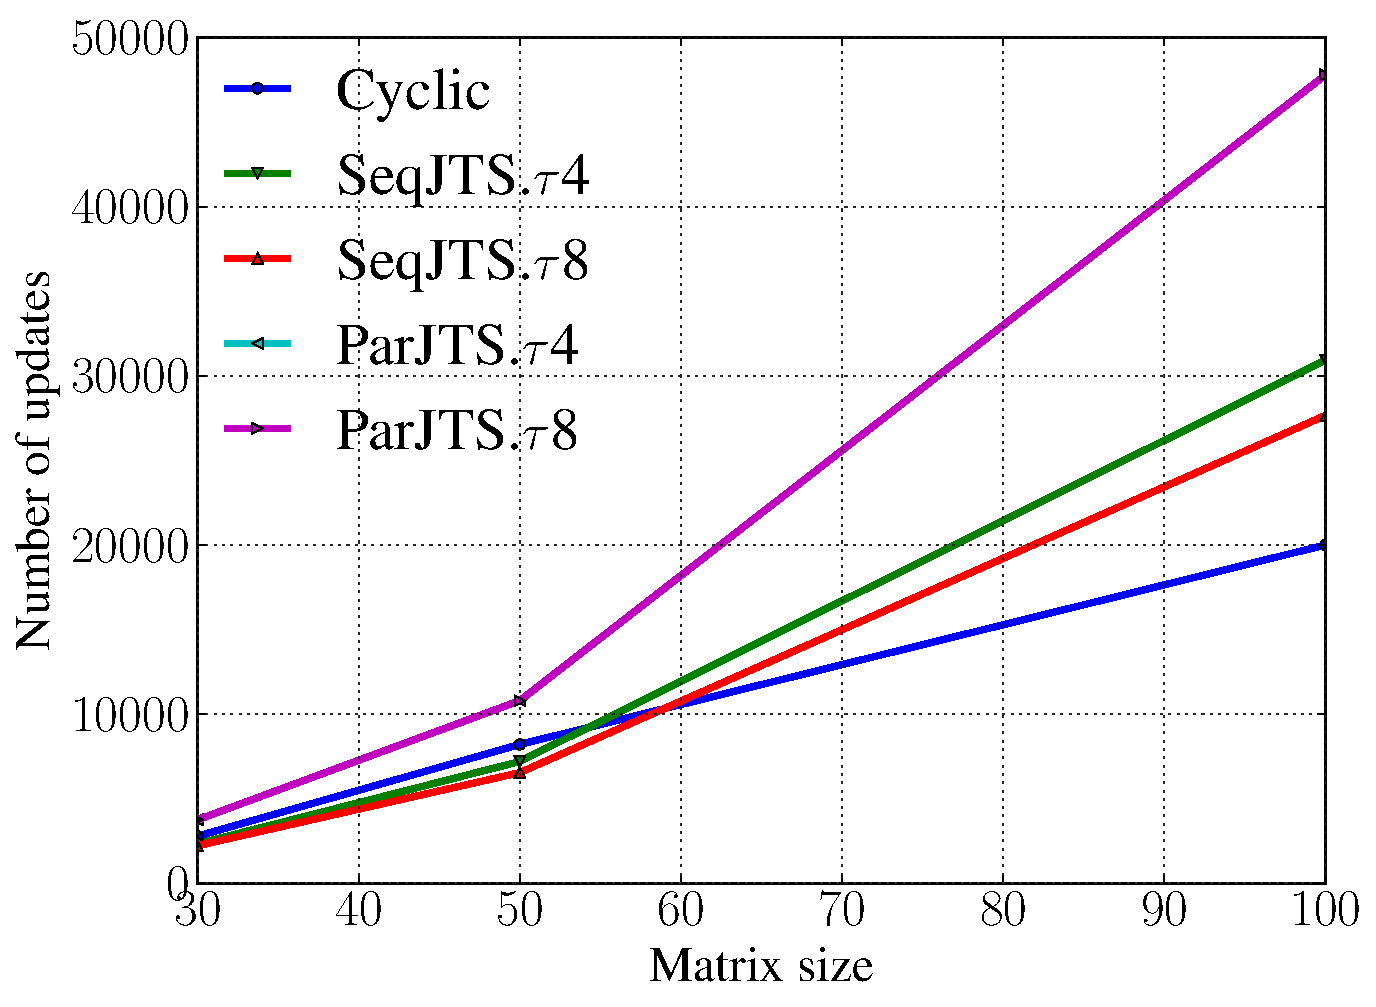
\includegraphics[width=0.31\textwidth]{updates}
 } \hfill
\subfloat[(b)][Time taken]{
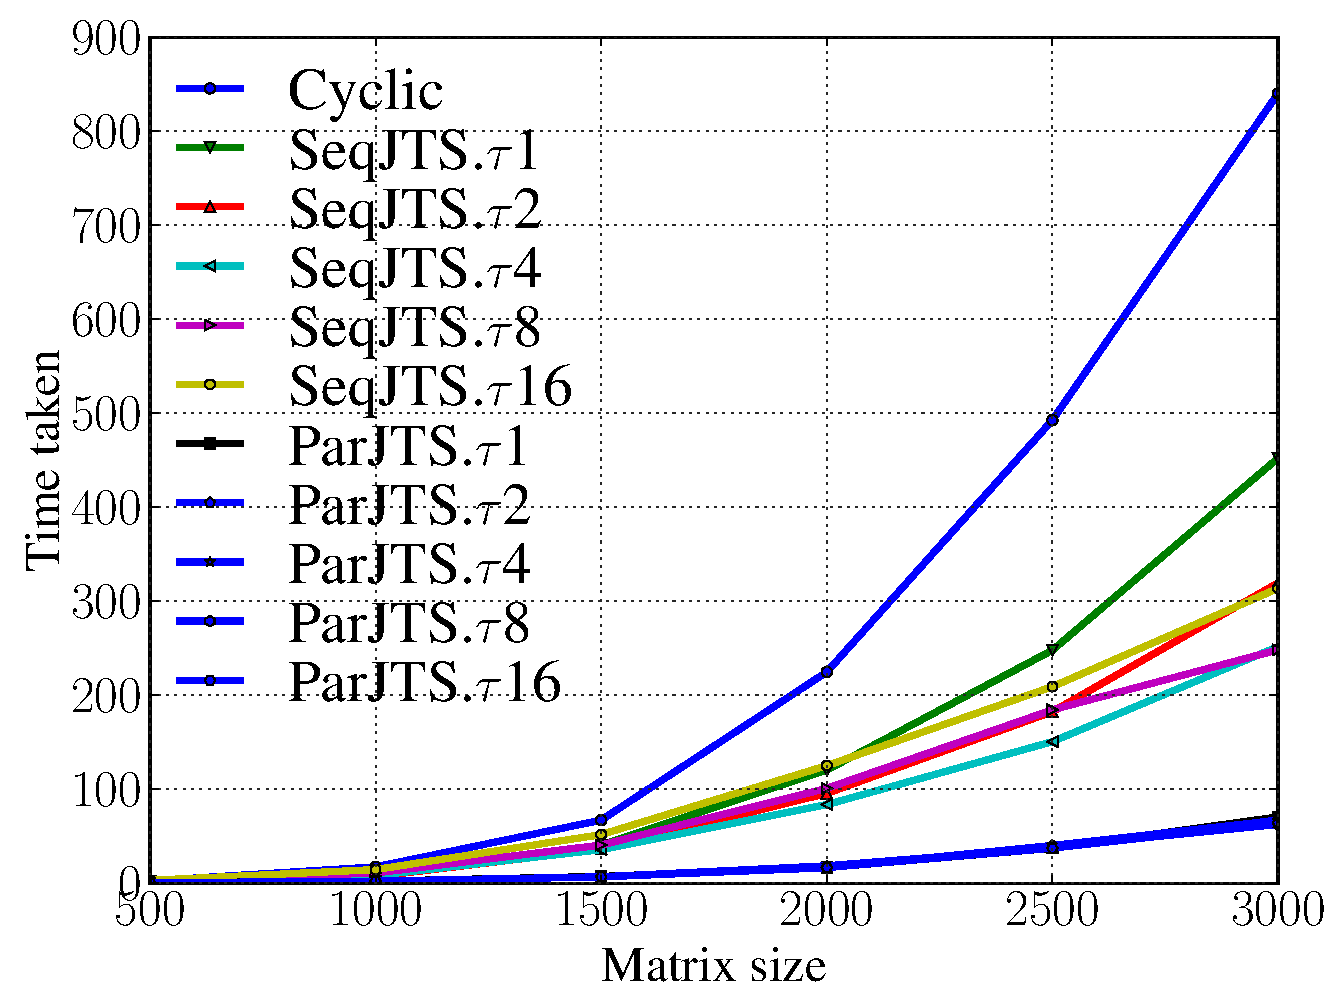
\includegraphics[width=0.31\textwidth]{timing}
 } \hfill
\subfloat[(b)][Scaling]{
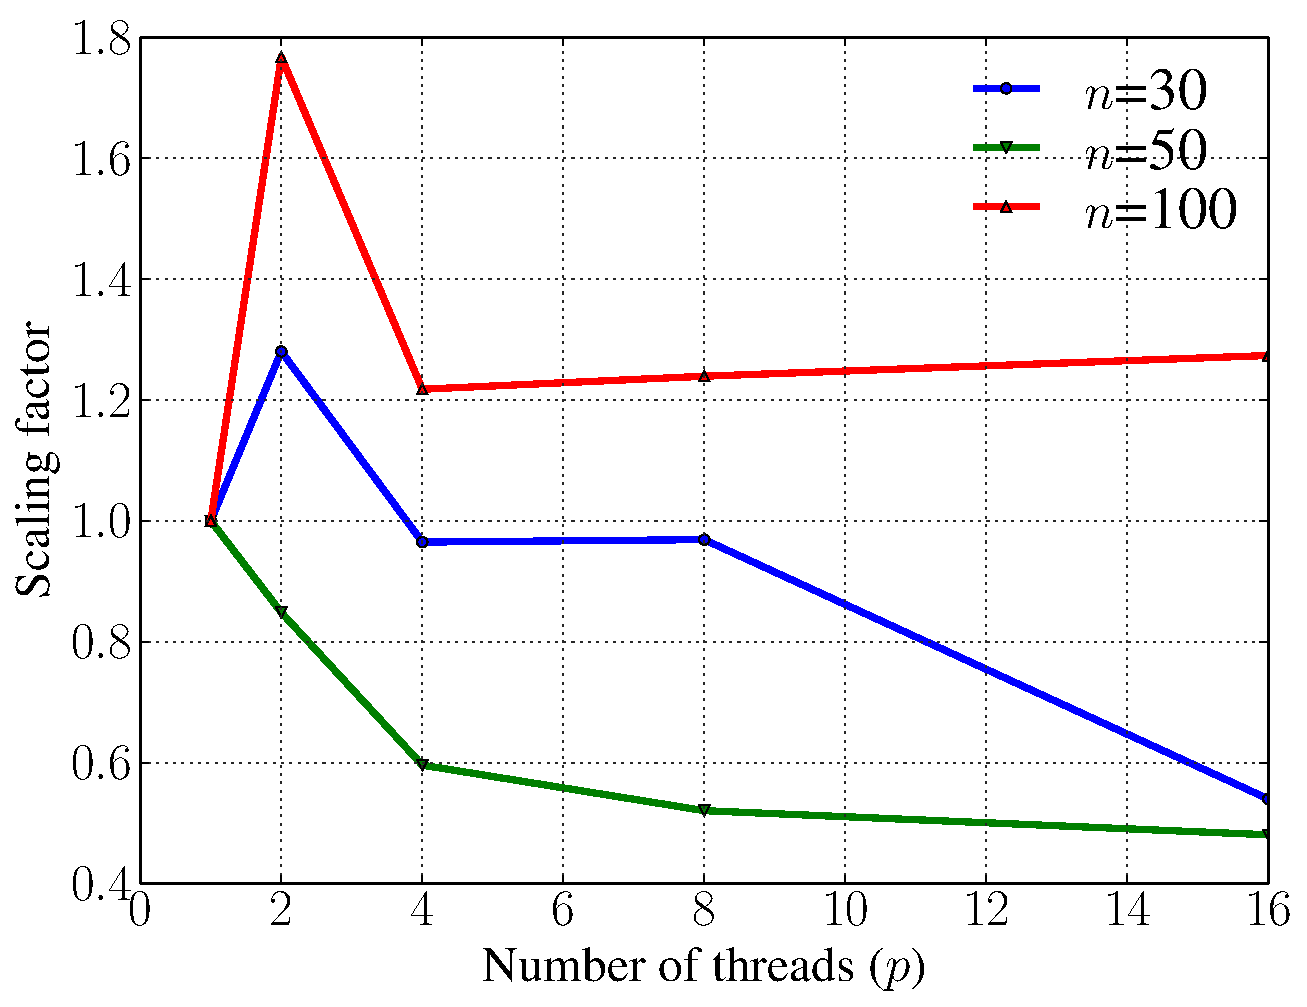
\includegraphics[width=0.31\textwidth]{scaling}
 }
\caption{Performance of real implementation of JTS}
\label{fig:real}
\end{figure*}

\section{Implementation on the PRAM and the Mesh}
\label{sec:other}

 In this section we implement JTS on various parallel models of computing including the PRAM and the mesh. A Parallel Random Access Machine (PRAM) is a collection of RAMs working in synchrony where communication takes place with the help of a common block of shared memory \cite{jaja1992introduction,horowitz2008computer}.  For instance if processor $i$ wants to communicate with processor $j$ it can do so by writing a message in memory cell $j$ which can then be read by processor $j$. More than one processor may want to either write into or read from the same cell at the same time. Depending on how these conflicts are handled, a PRAM can further be classified into three: Exclusive Read and Exclusive Write (EREW) PRAM, Concurrent Read and Exclusive Write (CREW) PRAM, and Concurrent Read and Concurrent Write (CRCW) PRAM.

%In the case of a CRCW PRAM, it is essential to have a mechanism for handling write conflicts, since the processors trying to write at the same time in the same cell can possibly have different data to write and we should determine which data gets written. This is not a problem in the case of concurrent reads since the data read by different processors will be the same. In a Common-CRCW PRAM, concurrent writes are permissible only if the processors trying to access the same cell have the same data to write.  In an Arbitrary-CRCW PRAM, if more than one processor tries to write in the same cell at the same time, an arbitrary one of them succeeds.  In a Priority-CRCW PRAM, processors have assigned priorities. Write conflicts are resolved using these priorities.

An $n \times n$ mesh can be represented as a directed $n\times n$ grid-graph whose nodes correspond to processing elements and whose edges correspond to bidirectional communication links \cite{leighton2014introduction,horowitz2008computer}.  If two processors are connected by an edge, they can communicate in a unit step. Otherwise, they communicate by sending a message along a connecting path.

% An $n\times n$ mesh is a $n\times n$ grid where each grid point corresponds to a processor and each edge corresponds to a (bidirectional link).

\subsection{Some Fundamental Parallel Algorithms}
In this section we  describe some basic algorithms that will be employed in the parallel implementation of JTS. These algorithms can be found in relevant texts (such as \cite{horowitz2008computer,jaja1992introduction,leighton2014introduction}).

Let $\oplus$ be any associative unit-time computable binary operator defined in some domain $\Sigma$. Given a sequence of $n$ elements $k_1,k_2,\ldots,k_n$ from $\Sigma$, the problem of {\em prefix computation} is to compute $k_1,k_1\oplus k_2,k_1\oplus k_2\oplus k_3,\ldots,k_1\oplus k_2\oplus\cdots \oplus k_n$.

\begin{lemma}
\label{prefix1}
Prefix computation on a sequence of $n$ elements can be performed in
$O(\log n)$ time using $n$ CREW PRAM processors.
\end{lemma}

\begin{lemma}
\label{prefix2}
Prefix computation on a sequence of $n^2$ elements can be performed in
$O(n)$ time on a $n\times n$ mesh. 
\end{lemma}

\begin{lemma}
\label{slowdown}
Any PRAM algorithm that runs in time $T$ using $P$ processors
can be simulated on a $P^\prime$-processor machine in time
$O\left (\frac{PT}{P^\prime}\right )$, for any $P^\prime\leq P$. \hfill $\Box$
\end{lemma}

\begin{lemma}
\label{sort1}
Any  sequence of arbitrary elements of length $n$ can be sorted in
$O(\log n)$ time using $n$ EREW PRAM processors.
\hfill $\Box$
\end{lemma}

\begin{lemma}
\label{sort2}
Any  sequence of arbitrary elements of length $n$ can be sorted in
$O( n)$ time using on a $n\times n$ mesh.
\hfill $\Box$
\end{lemma}

\subsection{Implementation on the PRAM}

For simplicity let the input matrix $A$ have size $n\times n$. The details of the parallel implementation of each of the three phases of a single sweep in Algorithm~\ref{algo:seqjts} are given below.


\noindent \textbf{Phase~1.} For a single pair of columns, the dot product can be computed in $O(\log n)$ time using $\frac{n}{\log n}$ CREW PRAM processors. For all pairs, it takes $O(\log n)$ time using a total of $\frac{n^3}{\log n}$ CREW PRAM processors. Sorting the ${n}\choose{2}$ dot product values and selecting the top ${n\choose 2}/\tau$ values takes $O(\log n)$ time using $n^2$ CREW PRAM processors.

\noindent \textbf{Phase~2.} For each of the pivot elements we have to compute a rotation matrix as in Equation~\eqref{eq:rotation} which can be done in $O(1)$ time. Thus phase~2 takes $O(1)$ time using $n^2$ processors.

\noindent \textbf{Phase~3.} After having computed all the ${n\choose 2}/\tau$ rotation matrices we have to multiply all of them. One possible way of doing this is to multiply each one of these matrices at a time with a cumulative product. Though the rotation matrix has only four nonzero entries, the cumulative product matrix can be possibly full. This multiplication can be done in $O(n)$ time sequentially. If we have a PRAM, this can be done in $O(1)$ time using $n$ processors. Thus phase~3 can be completed in $O(n^2)$ time using $n$ CREW PRAM processors. Alternatively, we can multiply all of these matrices like in a prefix computation. In this case each matrix multiplication can be between two possibly full matrices. Thus phase~3 can be completed in $O(\log^2n)$ time using $\frac{n^5}{\log n}$ processors.

Combining all three phases, we get the following result:

\begin{theorem}
The JTS algorithm has a parallel run-time of $O(S\log^2n)$ using $\frac{n^5}{\log n}$ CREW PRAM processors, and $O(Sn^2)$ using $n$ CREW PRAM processors. Here $S$ is the number of sweeps.
\end{theorem}

\subsection{Implementation on the Mesh}
We can run the JTS algorithm on the mesh as well. Phase~1 including sorting can be completed in $O(n)$ time on an $n\times n$ mesh. Phase~2 can be completed in $O(1)$ time, and phase~3 in $O(n^2)$ time. Thus, we get the following result.

\begin{theorem}
The JTS algorithm takes $O(Sn^2)$ time on an $n\times n$ mesh. Here $S$ is the number of sweeps.
\end{theorem}

\section{Conclusions}
\label{sec:conclude}

In this paper, we have proposed and implemented a novel algorithm (called JTS) for computing SVDs in parallel. JTS improves the number of sweeps required by applying only the top $\frac{1}{\tau}$ fraction of possible Jacobi rotations in a sweep (for some suitable value of $\tau$). We showed that our algorithm works better than known algorithms on both a simulated framework~\cite{rajasekaran2008relaxation} and a real implementation based on the code in GSL~\cite{galassi1996gnu}. We have also given theoretical results on the PRAM and the mesh. While experimenting on the real implementation we found that the cache misses play a big role as the selection of pivots and the application of rotations require computing dot-product of each column with all the others. In our future work, we would like to explore ideas from~\cite{haidar2013improved} and \cite{soliman2008memory} for a cache efficient implementation.

%% use section* for acknowledgement
%\section*{Acknowledgment}
%
%
%The authors would like to thank...
%more thanks here
%
%\begin{table}[!t]
%% increase table row spacing, adjust to taste
%\renewcommand{\arraystretch}{1.3}
% if using array.sty, it might be a good idea to tweak the value of
% \extrarowheight as needed to properly center the text within the cells
%\caption{An Example of a Table}
%\label{table_example}
%\centering
%% Some packages, such as MDW tools, offer better commands for making tables
%% than the plain LaTeX2e tabular which is used here.
%\begin{tabular}{|c||c|}
%\hline
%One & Two\\
%\hline
%Three & Four\\
%\hline
%\end{tabular}
%\end{table}


% Note that IEEE does not put floats in the very first column - or typically
% anywhere on the first page for that matter. Also, in-text middle ("here")
% positioning is not used. Most IEEE journals/conferences use top floats
% exclusively. Note that, LaTeX2e, unlike IEEE journals/conferences, places
% footnotes above bottom floats. This can be corrected via the \fnbelowfloat
% command of the stfloats package.



% trigger a \newpage just before the given reference
% number - used to balance the columns on the last page
% adjust value as needed - may need to be readjusted if
% the document is modified later
%\IEEEtriggeratref{8}
% The "triggered" command can be changed if desired:
%\IEEEtriggercmd{\enlargethispage{-5in}}

% references section

\balance

% can use a bibliography generated by BibTeX as a .bbl file
% BibTeX documentation can be easily obtained at:
% http://www.ctan.org/tex-archive/biblio/bibtex/contrib/doc/
% The IEEEtran BibTeX style support page is at:
% http://www.michaelshell.org/tex/ieeetran/bibtex/
\bibliographystyle{IEEEtran}
% argument is your BibTeX string definitions and bibliography database(s)
\small
\def\IEEEbibitemsep{1.5pt plus .5pt}
\bibliography{IEEEabrv,jacobi}


% that's all folks
\end{document}


